\section{Control Supervisado}
{\begin{small}%
\begin{flushright}%
\it
Entiende el problema y tendrás la solución
\end{flushright}%
\end{small}%
\vspace{.5cm}}
El presente proyecto de tesis consistió en un estudio y extensión del método previamente propuesto por Daniel Ciolek en su tesis de doctorado[REF PAPER?]. Más precisamente, se trató de analizar carencias del algoritmo de exploración on-the-fly para problemas de Supervisory Control, cuya propiedad central era de tipo Non-blocking, y posteriormente analizados los problemas afrontarlos con una nueva especificación e implementación del algoritmo.
\\
Un problema de Control Supervisado consiste en un Sistema de Eventos Discreto (DES) con un subconjunto de sus estados marcados. Un factor clave de estos problemas es que el DES se presenta de forma compacta, de forma modular tal que la composición paralela de múltiples componentes den lugar a la DES de interés.
\\

\subsection{Caso de estudio}
A continuación se presenta un ejemplo sobre el cual aplicaremos nuestro algoritmo a lo largo de la presentación. 

Imaginemos un negocio del cual modelamos 3 componentes: La cuenta de dinero, la estación de ventas de productos terminados, y la estación de compra de materia prima y ensamblaje de productos.

La cuenta de dinero puede estar vacía o con dinero, no contamos cuanto dinero hay, pero sabemos que en caso de estar vacía no se pueden comprar nuevas materias primas. También podemos elegir al momento de comprar nuevos materiales si queremos gastar todo el dinero que hay en la cuenta o solo gasta una parte.

La estación de ensamble puede necesitar comprar nuevos materiales, y una vez que los recibe necesita un tiempo no controlable hasta finalizar el próximo producto, momento en el que el mismo se transfiere a la estación de ventas.

La estación de ventas, cuando tiene un producto para vender, tarda un tiempo no controlable hasta que llega un cliente que compra el producto, momento en el que la cuenta del negocio guarda la plata y seguramente no está vacía.

Mostramos en la figura~\ref{fig:modelos} un LTS (Labeled transition system) para cada uno de los componentes descriptos.


\begin{figure}[htb]
	\begin{center}
	\makebox[\linewidth][c]{%
	\begin{subfigure}[t]{.7\textwidth}
		\centering
		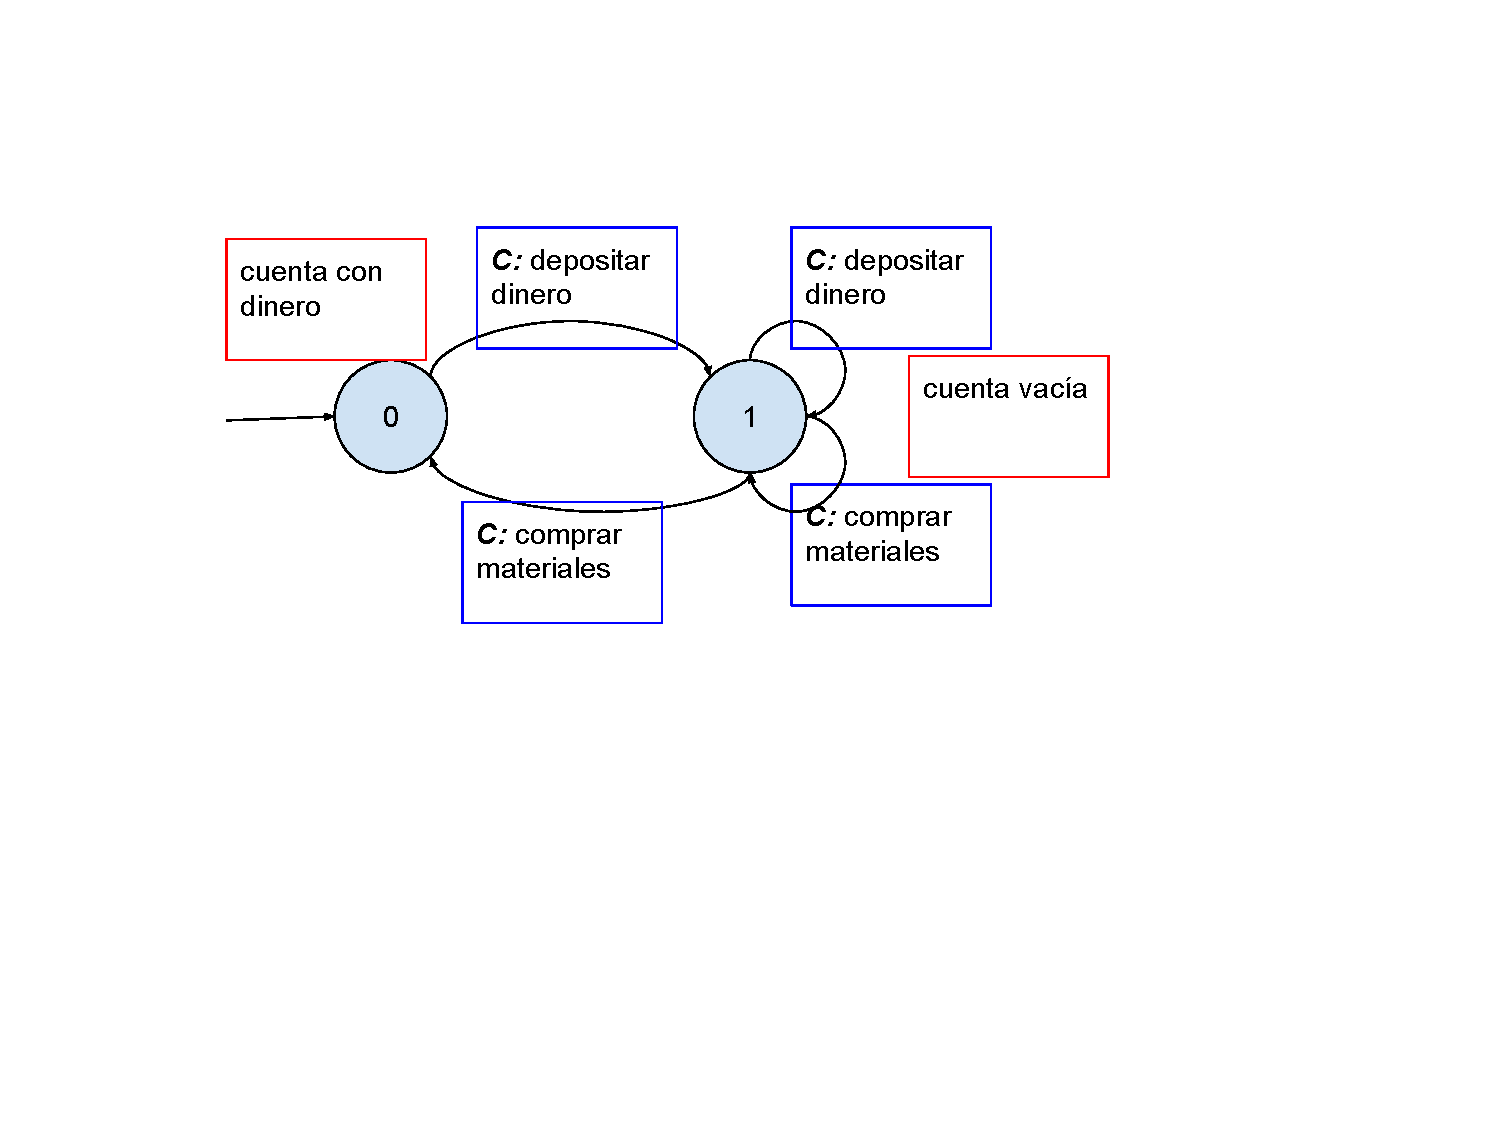
\includegraphics[width=\linewidth]{figures/ModeloCuentaBanco.pdf}  
		\caption{Cuenta bancaria}
		\label{fig:ModeloBanco}
	\end{subfigure}
	\begin{subfigure}[t]{.7\textwidth}
		\centering
		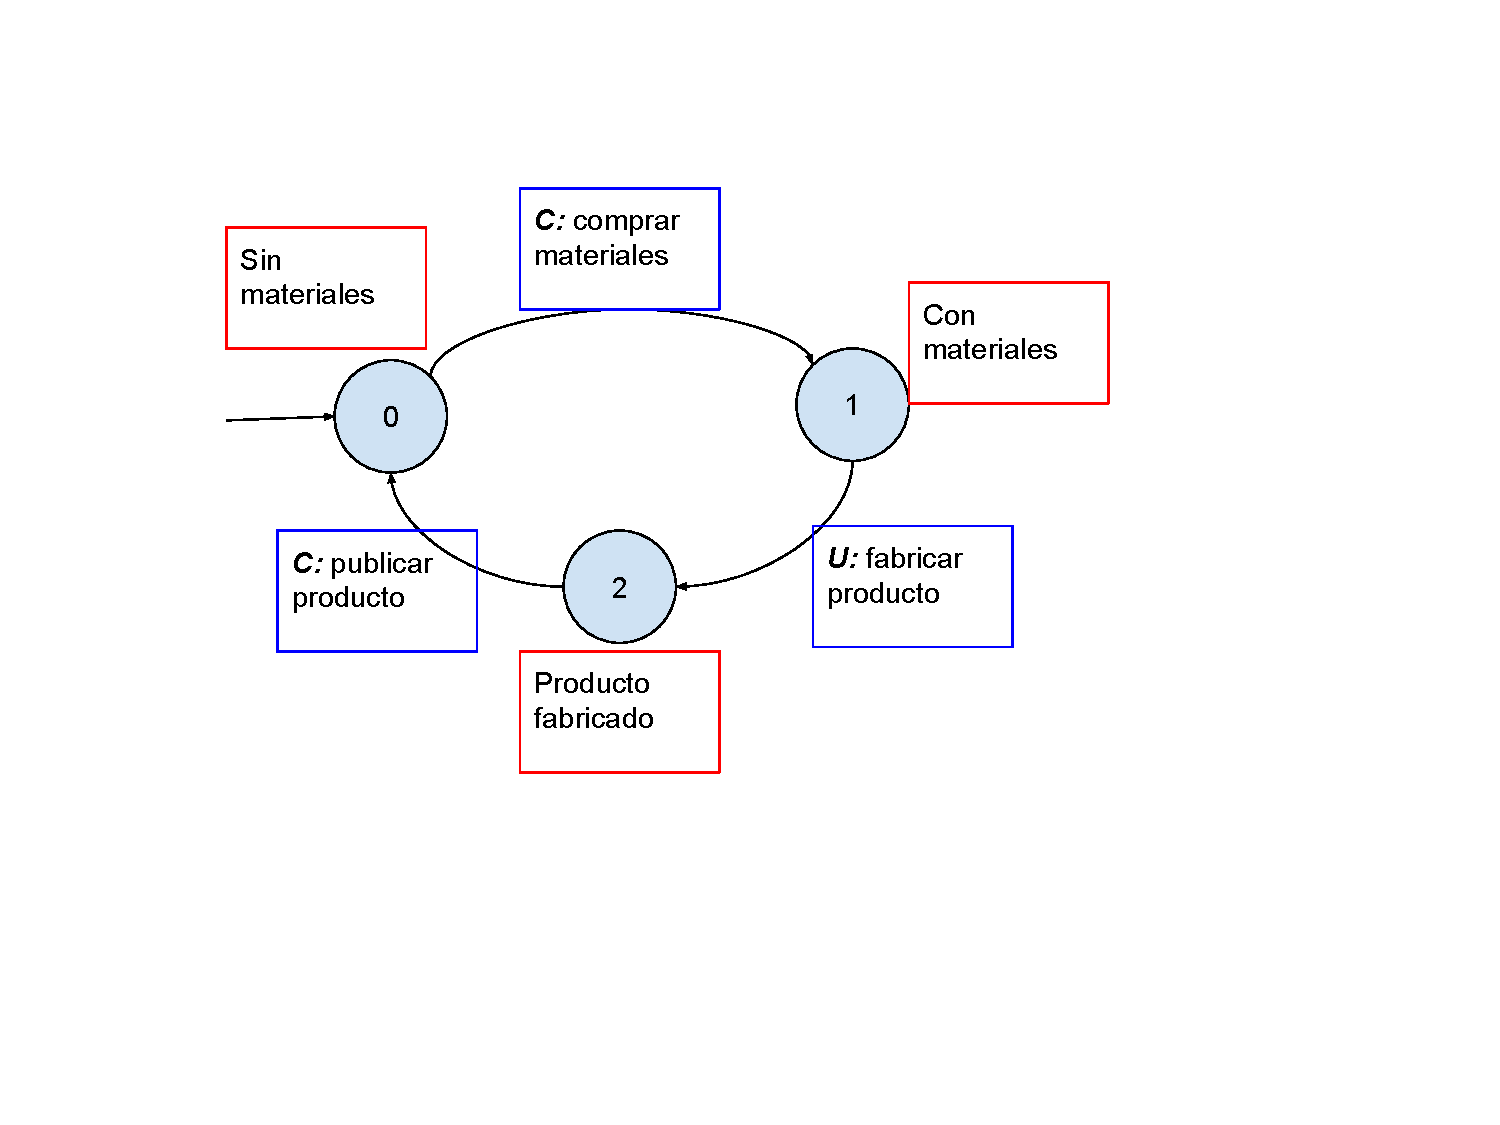
\includegraphics[width=\linewidth]{figures/ModeloEnsamblaje.pdf}  
		\caption{Estacion de ensamblaje}
		\label{fig:modeloEnsamblajes}
	\end{subfigure}
	}
	\makebox[\linewidth][c]{%
	\begin{subfigure}[t]{.7\textwidth}
		\centering
		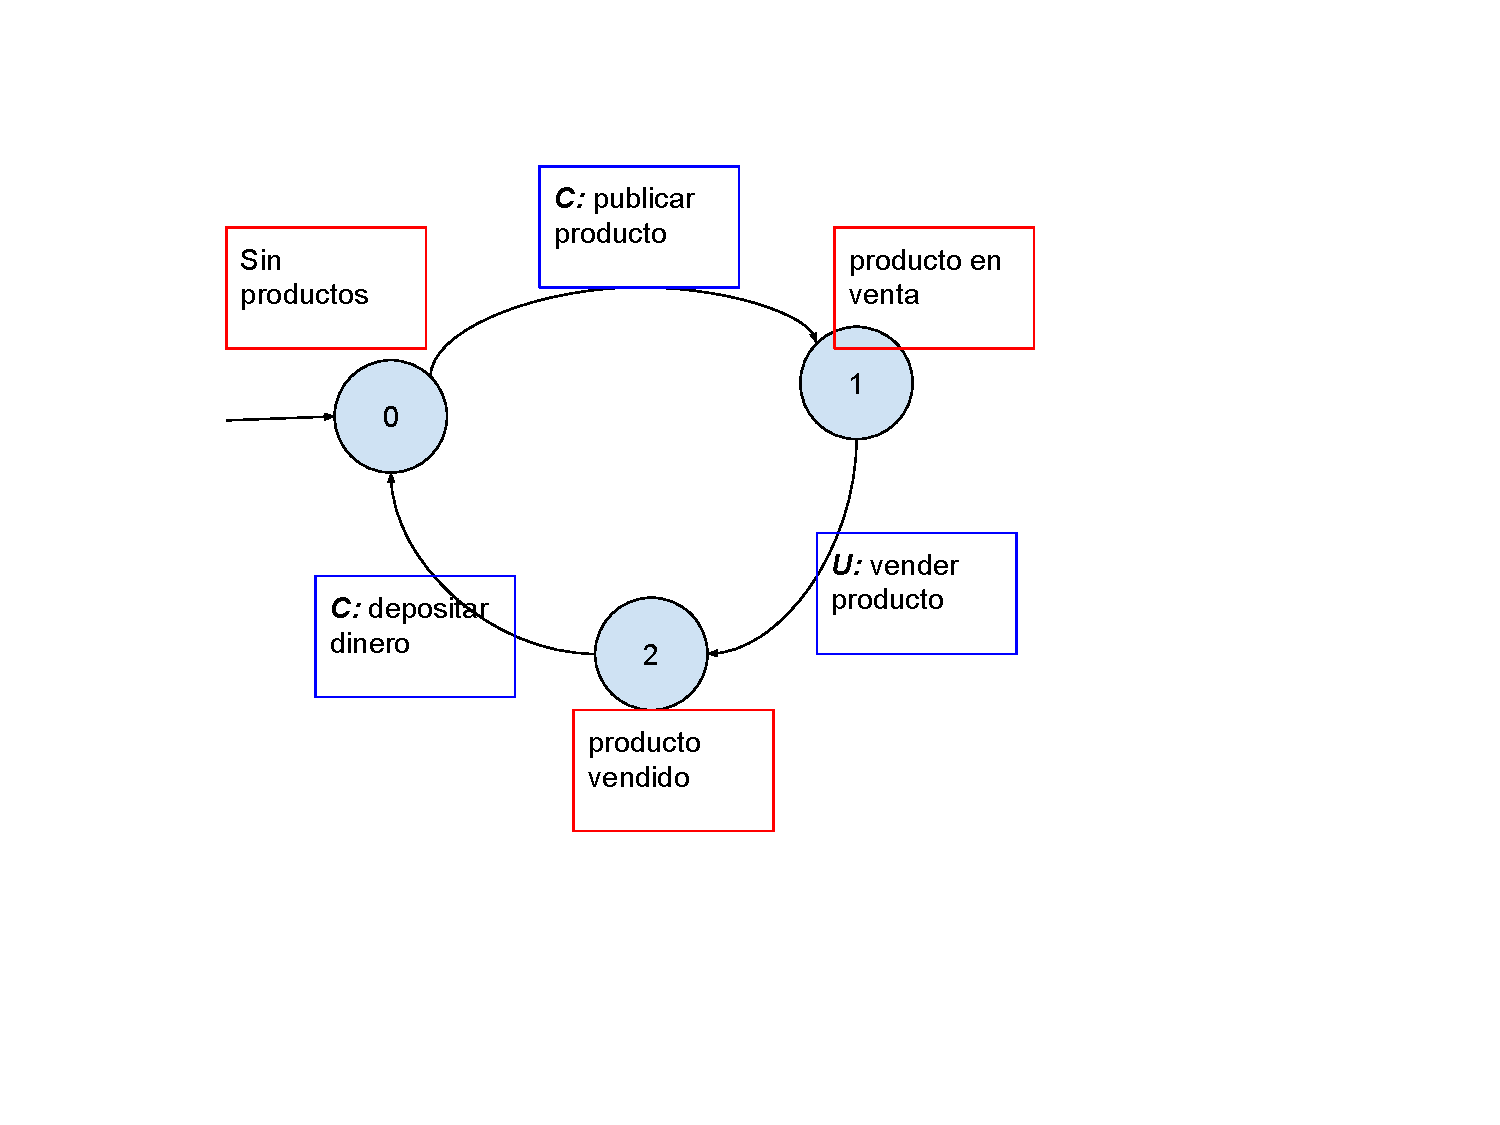
\includegraphics[width=\linewidth]{figures/ModeloVentas.pdf}  
		\caption{Estacion de ventas}
		\label{fig:modeloVentas}
	\end{subfigure}
	\begin{subfigure}[t]{.7\textwidth}
	\centering
	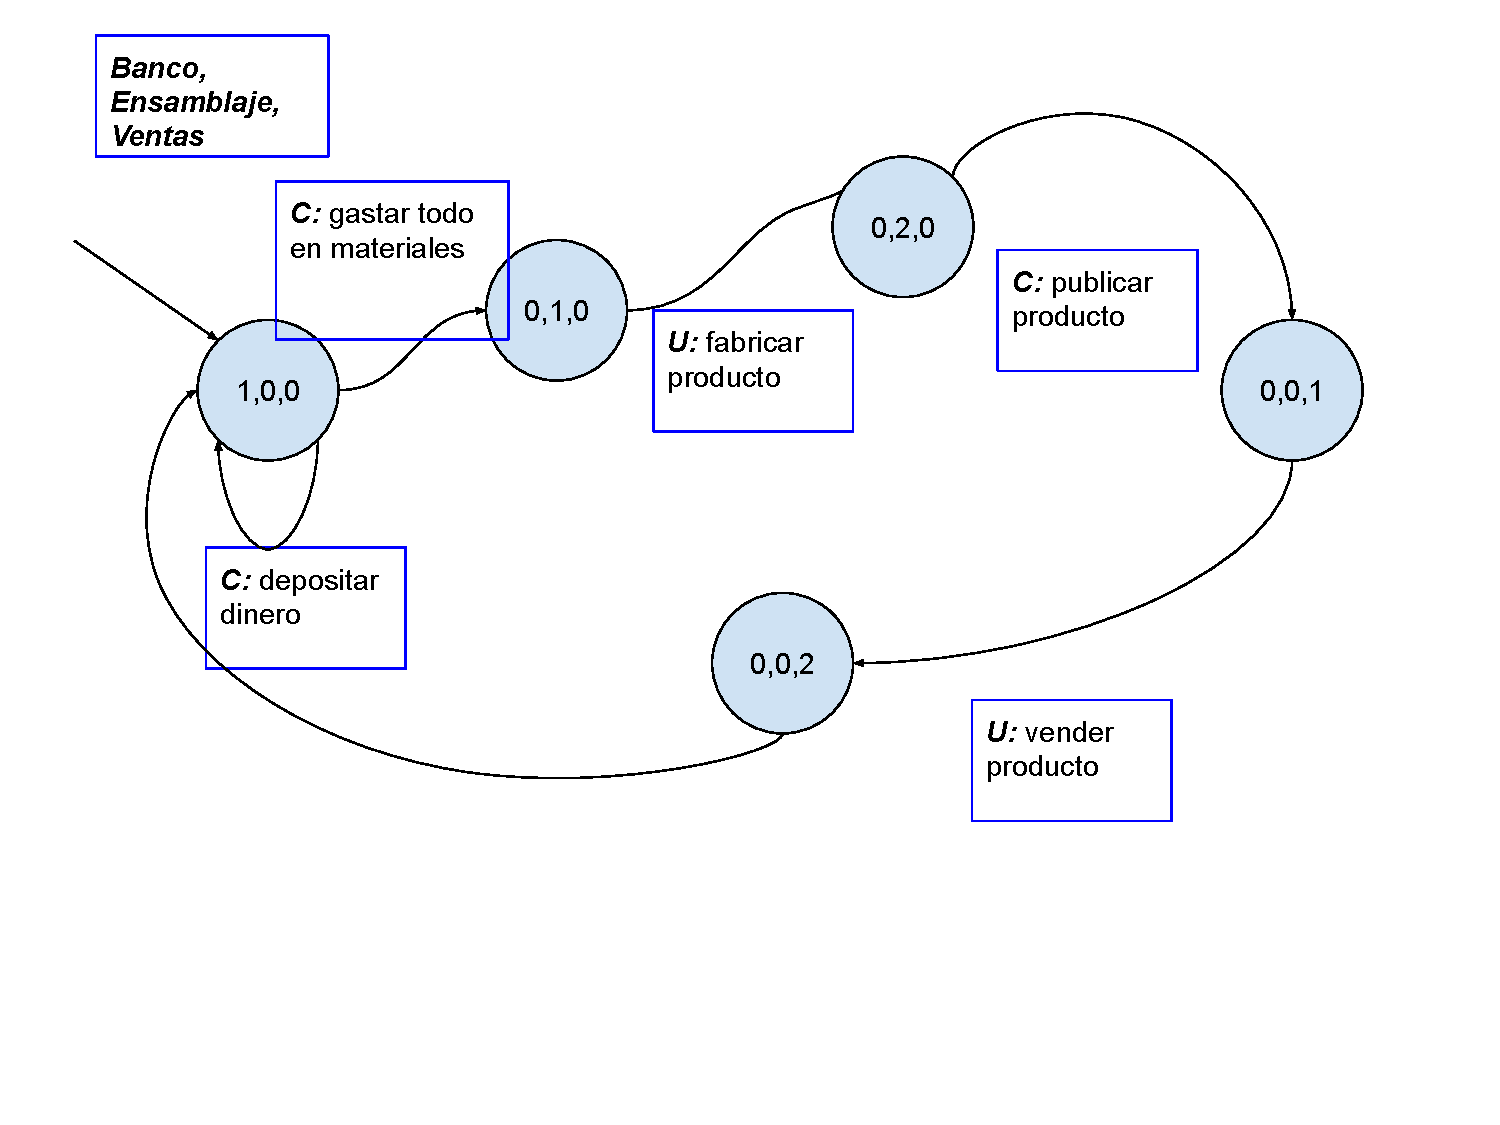
\includegraphics[width=\linewidth]{figures/ModeloCompuestoSin2Caminos.pdf}  
	\caption{Composición de los componentes}
	\label{fig:compuesto}
	\end{subfigure}
	}
	\caption{Modelo de ejemplo}
	\label{fig:modelos}
	\end{center}
\end{figure}



\subsection{Controlador objetivo}
El problema a tratar consiste en encontrar para la planta de entrada, un controlador, es decir, un autómata con las siguientes características:

	-Es sub-autómata de la planta: todos los estados y transiciones del controlador existen en la planta compuesta.
	-Es controlable: todas las transiciones no controlables de la planta se encuentran en el controlador.
	-Es non-blocking: cada palabra válida para el controlador puede ser extendida por otra palabra no vacía para que su concatenación alcance un estado marcado.
	
Podemos pensar en un controlador non-blocking como un jugador optimista. Se encarga de no perder, y mientras tenga un futuro camino posible que lo lleva al destino buscado, considera que está ganando.

Es clave entender que en el problema a tratar, la posición de "tablas" del ajedrez, en la que ambos jugadores repiten sus jugadas 50 veces, se considera ganadora si todavía hay opción de dar un jaque mate. Si repetimos nuestras jugadas y todavía tengo dos torres considero que gané el partido, porque eventualmente mi oponente podría cansarse y dejarme ganar. Si repetimos nuestras jugadas pero solo tengo mi rey, no hay forma de dar mate, no puedo extender esta "palabra", esta partida, de forma de dar mate, y considero que perdí.

Es importante notar que como se busca que cualquier palabra sea extendible a otro estado marcado, lo que se busca es pasar por algún estado marcado infinitas veces. O sea, un estado "e" marcado que tenga un camino para que el jugador pueda volver controlablemente al mismo estado "e".

Por esto, las estructuras claves que analizamos en nuestro algoritmo son los "loops", ya que los primeros estados ganadores son aquellos que están en un loop controlable con un estado marcado dentro. Luego señalizamos como ganadores también a cualquier estado que controlablemente alcanza un estado ganador.

También los "loops" son esenciales para encontrar los estados perdedores, ya que la única forma de que un estado sea perdedor es que no pueda alcanzar un estado ganador. En otras palabras, los estados perdedores son aquellos que forman parte de un loop que no tiene estados marcados ni transiciones salientes.

De forma más concreta, en nuestro algoritmo, un "loop" del cual el jugador no puede escapar, pero desde el cual existe un camino hacia un estado ganador, se considera ganador.
\\

\subsection{Exploración on-the-fly}
Problema explosión exponencial: Componer todo vs BFS
\\



















